\documentclass[12pt,a4paper,austrian]{article}
\usepackage{graphicx}
\usepackage[austrian, english]{babel}
\usepackage[utf8]{inputenc}
%\usepackage{listings}
\usepackage{multirow}
\usepackage{epstopdf}
\usepackage{amsmath}
\usepackage{amssymb}
\usepackage{hyperref} % fuer Mengen \N, Q, C, R
\graphicspath{{./fig/}}


%% Satzspiegel
\setlength{\hoffset}{-1in} \setlength{\textwidth}{18cm}
\setlength{\oddsidemargin}{1.5cm}
\setlength{\evensidemargin}{1.5cm}
\setlength{\marginparsep}{0.7em}
\setlength{\marginparwidth}{0.5cm}

\setlength{\voffset}{-1.9in}
\setlength{\headheight}{12pt}
\setlength{\topmargin}{2.6cm}
   \addtolength{\topmargin}{-\headheight}
\setlength{\headsep}{3.5cm}
   \addtolength{\headsep}{-\topmargin}
   \addtolength{\headsep}{-\headheight}
\setlength{\textheight}{27cm}

%% How should floats be treated?
\setlength{\floatsep}{12 pt plus 0 pt minus 8 pt}
\setlength{\textfloatsep}{12 pt plus 0pt minus 8 pt}
\setlength{\intextsep}{12 pt plus 0pt minus 8 pt}

\tolerance2000
\emergencystretch20pt

%% Text appearence
% English text
\newcommand{\eg}[1]%
  {\selectlanguage{english}\textit{#1}\selectlanguage{austrian}}

\newcommand{\filename}[1]
  {\begin{small}\texttt{#1}\end{small}}

\newcommand\IFT{\unitlength1mm\begin{picture}(10,2) \put (1,1)
{\circle{1.7}} \put(2,1){\line(1,0){5}} \put(8,1)
{\circle*{1.7}}\end{picture}}
\newcommand\FT{\unitlength1mm\begin{picture}(10,2) \put (1,1)
{\circle*{1.7}} \put(2,1){\line(1,0){5}} \put(8,1)
{\circle{1.7}}\end{picture}}

% A box for multiple choice problems
\newcommand{\choicebox}{\fbox{\rule{0pt}{0.5ex}\rule{0.5ex}{0pt}}}

\newenvironment{wahrfalsch}%
  {\bigskip\par\noindent\makebox[1cm][c]{richtig}\hspace{3mm}\makebox[1cm][c]{falsch}
   \begin{list}%
   {\makebox[1cm][c]{\choicebox}\hspace{3mm}\makebox[1cm][c]{\choicebox}}%
   {\setlength{\labelwidth}{2.31 cm}\setlength{\labelsep}{3mm}
    \setlength{\leftmargin}{2.61 cm}\setlength{\listparindent}{0pt}
    \setlength{\itemindent}{0pt}}%
  }
  {\end{list}}

\newcounter{theaufgabe}\setcounter{theaufgabe}{1}
\newenvironment{aufgabe}[1]%
  {\bigskip\par\noindent\begin{nopagebreak}
   \textsf{\textbf{\arabic{theaufgabe}.\thinspace Aufgabe}}\quad
      \textsf{\textit{#1}}\\*[1ex]%
\stepcounter{theaufgabe}\hspace{2ex}\end{nopagebreak}}
  {\par\pagebreak[2]}

% Innerhalb der Aufgaben erfolgt die weitere Unterteilung mittels einer
% enumerate Umgebung, die allerdings a), b),... zaehlen soll.
\renewcommand{\labelenumi}{\alph{enumi})}
\renewcommand{\labelenumii}{\arabic{enumii})}

% A box to tick for everything which has to done
\newcommand{\abgabe}{\marginpar{$\Box$}}
% Margin paragraphs on the left side
\reversemarginpar

% Language for listings
%\lstset{language=Vhdl,
%  basicstyle=\small\tt,
 % keywordstyle=\tt\bf,
 % commentstyle=\sl}

% No indention
\setlength{\parindent}{0.0cm}
% Don't number sections
\setcounter{secnumdepth}{0}


%% Beginning of the text

\begin{document}
\selectlanguage{austrian}
\pagestyle{plain}


%===  This is the header section ============================================================
\thispagestyle{empty}
\noindent
\begin{minipage}[b][4cm]{1.0\textwidth}  
\begin{center}
\begin{bf} 
\begin{large} Digital Signal Processing SS 2024 -- 3.~Assignment\end{large} \\
\vspace{0.3cm}
\begin{Large} Sampling and Reconstruction \end{Large} \\
\vspace{0.3cm}
\end{bf}
\begin{large}
Group 22\\
Julian Feichtinger, K12015812\\
Wolfram Laube, K08900915\\
\end{large} 
\end{center}
\end{minipage}

\noindent \rule[0.8em]{\textwidth}{0.12mm}\\[-0.5em]
%=======================================================================================


\begin{aufgabe}{Sampling 1 (40\%)}

The analogue signal

\[
x(t) = x_{1}(t) + x_{2}(t) = \sin \left(2 \pi f_{1} t\right) + \sin \left(2 \pi f_{2} t\right)
\]

with \(f_{1} = 4 \mathrm{kHz}\) and \(f_{2} = 6 \mathrm{kHz}\) is sampled with a sampling rate of \(f_{s} = 10 \mathrm{kHz}\) to yield the discrete time signal \(x[n]\).

\begin{enumerate}
    \item[(a)] Draw the spectrum of \(x(t)\).

    \item[(b)] Due to sampling frequency shifted versions of the analogue spectrum are generated.

    Draw the spectra shifted by \(-f_{s}, 0\) and \(+f_{s}\) and then the spectrum for \(x[n]\) as a result of spectral addition in one diagram.
    The diagram should show the spectra in the range from \(-f_{s}\) to \(+f_{s}\).

    \emph{Hint: Draw real and imaginary parts of the spectrum rather than magnitude and phase to ease addition.}

    \item[(c)] In Matlab, plot the section 0 to \(2 \mathrm{~ms}\) of the signal \(x(t)\) with a sampling rate of \(100 \mathrm{kHz}\) to emulate an analogue signal.

    Then also add the sampled signal \(x[n] = x\left(n T_{s}\right)\) to the same plot.
    Show that \(x[n]\) corresponds to the spectrum derived in (b).
\end{enumerate}


\hrule
\begin{enumerate}
%! Author = wolfram_e_laube
%! Date = 17.04.24

\item[(a)]
The discrete time signals are plotted with the appropriate commands to display the nature of the signals.
For the signals $x_{1}[n]$ and $x_{2}[n]$, the stem command is used to emphasize their discrete nature,
and for the longer signals $x_{3}[n]$ and $x_{4}[n]$, the plot command is utilized.

\begin{verbatim}
% Define the sample ranges
n1 = -5:10;
n2 = 0:256;

% Define the signals
x1 = -4 * (n1 == -3) + 4 * (n1 == 0) - (n1 == 3) + 2 * (n1 == 7);
x2 = exp(-0.31 * n1);
x3 = 3 * sin(2 * pi * 3.5/64 * n2);
x4 = -cos(9/64 * n2);

% Plot the signals
figure;
subplot(2,2,1);
stem(n1, x1, 'filled');
title('Signal x1[n]');

subplot(2,2,2);
stem(n1, x2, 'filled');
title('Signal x2[n]');

subplot(2,2,3);
plot(n2, x3);
title('Signal x3[n]');

subplot(2,2,4);
plot(n2, x4);
title('Signal x4[n]');
\end{verbatim}

%! Author = wolfram_e_laube
%! Date = 06.05.24

\item[(b)]
\section{Task (b): Fourier Transform and Spectrum Visualization}

\subsection{Fourier Transform of $x(t)$}
Given the signal $x(t) = \sin(2\pi 4000 t) + \sin(2\pi 6000 t)$, we calculate the Fourier transform, which reveals delta functions at the frequencies of the sinusoidal components:
$$
X(f) = \frac{1}{2i} \left(\delta(f - 4000) - \delta(f + 4000) + \delta(f - 6000) - \delta(f + 6000)\right)
$$
This expression indicates that the spectrum of $x(t)$ consists of spikes at $\pm 4000$ Hz and $\pm 6000$ Hz.

\subsection{Spectrum Visualization and Sampling Effects}
The spectrum is then visualized, taking into account the sampling frequency $f_s = 10,000$ Hz, which leads to periodic replication of the spectrum. The replication and the combination of these spectra due to sampling are illustrated to show how aliasing could affect the resultant digital signal $x[n]$. The effects are demonstrated using a Python script that plots the original and shifted spectra within the range $-f_s$ to $+f_s$.

\begin{figure}[h]
    \centering
    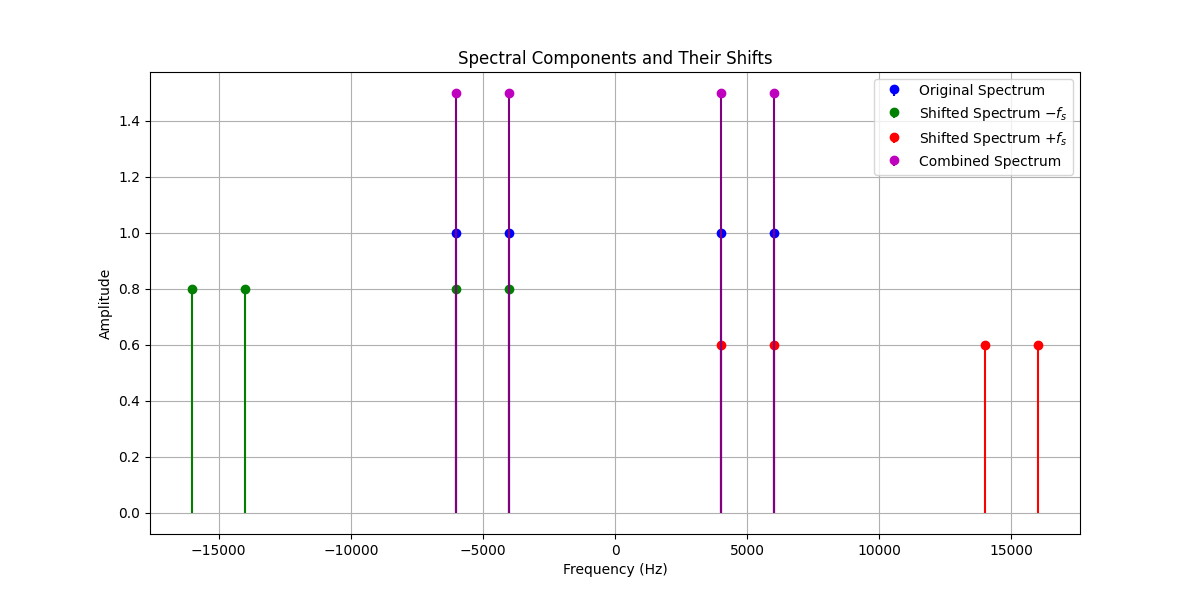
\includegraphics[width=0.49\textwidth]{fig/ex1_b_plot}
    \caption{Spectrum of \(x(t)\)}
    \label{fig:ex1_b_plot}
\end{figure}

The shifted spectrum plot will show the spectral shifts due to the sampling frequency and illustrate the overlapping spectra.
%! Author = wolfram_e_laube
%! Date = 06.05.24

\item[(c)]
The Python code accomplishing this is:

\begin{verbatim}
import numpy as np
import matplotlib.pyplot as plt

# Parameters
fs_analog = 100e3  # 100 kHz
fs = 10e3  # 10 kHz
f1 = 4e3  # 4 kHz
f2 = 6e3  # 6 kHz
t_end = 2e-3  # 2 ms

# Time vectors
t = np.arange(0, t_end, 1/fs_analog)
n = np.arange(0, int(t_end * fs))

# Analog signal
x_t = np.sin(2 * np.pi * f1 * t) + np.sin(2 * np.pi * f2 * t)

# Sampled signal
x_n = np.sin(2 * np.pi * f1 * n / fs) + np.sin(2 * np.pi * f2 * n / fs)

# Plotting
plt.figure()
plt.plot(t * 1e3, x_t, label='Analog signal x(t)')
plt.stem(n * 1e3 / fs, x_n, linefmt='r', markerfmt='ro', basefmt=' ', label='Sampled signal x[n]', use_line_collection=True)
plt.xlabel('Time (ms)')
plt.ylabel('Amplitude')
plt.title('Analog and Sampled Signals')
plt.legend()
plt.grid(True)
plt.show()
\end{verbatim}

\begin{figure}[h]
    \centering
    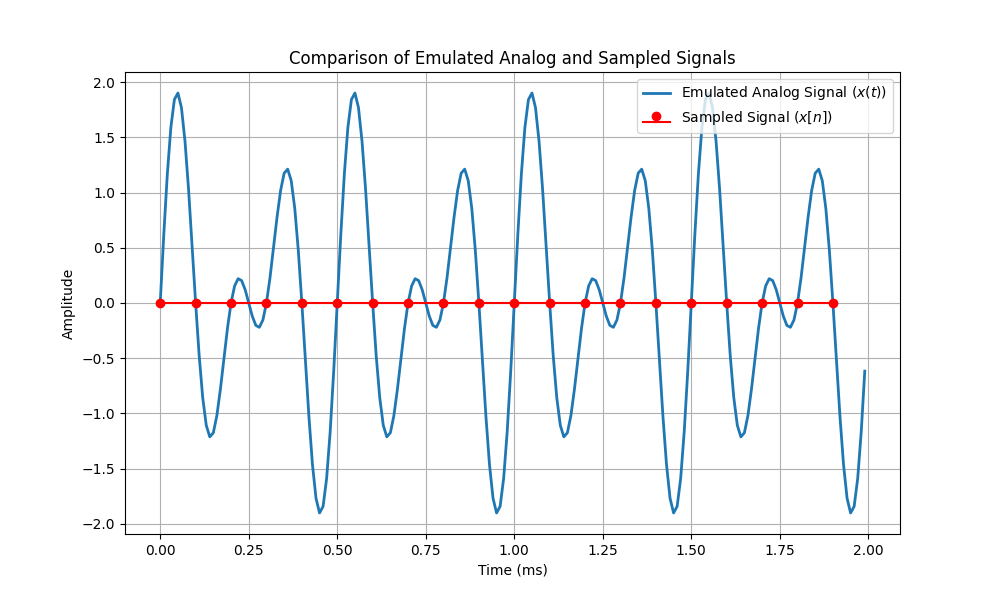
\includegraphics[width=0.49\textwidth]{fig/ex1_c_plot}
    \caption{Analog and Sampled Signals of \(x(t)\)}
    \label{fig:ex1_c_plot}
\end{figure}

\end{enumerate}

\end{aufgabe}

\begin{aufgabe}{Sampling 2 (25\%)}

The spectrum \(X(f)\) of an analogue signal \(x(t)\) is given with:

\begin{figure}[h]
    \centering
    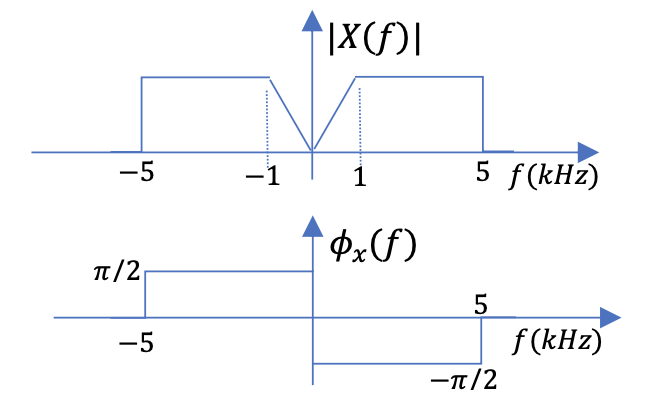
\includegraphics[width=0.49\textwidth]{fig/ex2_signal_spectrum}
    \caption{Spectrum of \(x(t)\)}
    \label{fig:ex2_signal_spectrum}
\end{figure}

\begin{enumerate}
    \item[(a)] Draw the real and imaginary parts of the spectrum \(X(f)\).

    \item[(b)] \(x(t)\) is sampled with \(8 \mathrm{kHz}\) to yield the discrete time signal \(x[n]\).
    Draw the spectrum of \(x[n]\) from \(-f_{s}\) to \(f_{s}\) and indicate the baseband.

\end{enumerate}

\hrule

\begin{enumerate}
%! Author = wolfram_e_laube
%! Date = 06.05.24

\item[(a)]
\subsection{Task (a): Real and Imaginary Parts of $X(f)$}

\subsubsection{Problem Statement}
Visualize the real and imaginary components of the frequency spectrum $X(f)$, given its magnitude $|X(f)|$ and phase $\phi_x(f)$, and discuss the implications of these components in signal processing.

\subsubsection{Mathematical Formulation}
Given:
\begin{itemize}
    \item \textbf{Magnitude $|X(f)|$:}
    \[
    |X(f)| =
    \begin{cases}
    A & \text{if } -5 \leq f < -1 \text{ or } 1 < f \leq 5 \\
    A(1 + f) & \text{if } -1 \leq f < 0 \\
    A(1 - f) & \text{if } 0 \leq f \leq 1 \\
    0 & \text{otherwise}
    \end{cases}
    \]

    \item \textbf{Phase $\phi_x(f)$:}
    \[
    \phi_x(f) =
    \begin{cases}
    \frac{\pi}{2} & \text{if } -5 \leq f < 0 \\
    -\frac{\pi}{2} & \text{if } 0 < f \leq 5 \\
    0 & \text{otherwise}
    \end{cases}
    \]
\end{itemize}

Using Euler's formula:
\[
X(f) = |X(f)| \cdot e^{i \phi_x(f)}
\]
\[
\text{Re}\{X(f)\} = |X(f)| \cos(\phi_x(f))
\]
\[
\text{Im}\{X(f)\} = |X(f)| \sin(\phi_x(f))
\]

\subsubsection{Discussion}
The real part $\text{Re}\{X(f)\}$ is zero for all $f$, reflecting the phase shifts of $\frac{\pi}{2}$ and $-\frac{\pi}{2}$. The imaginary part $\text{Im}\{X(f)\}$ shows variations with $f$, mirroring the magnitude adjustments and the sinusoidal phase behavior.

\begin{figure}[h]
    \centering
    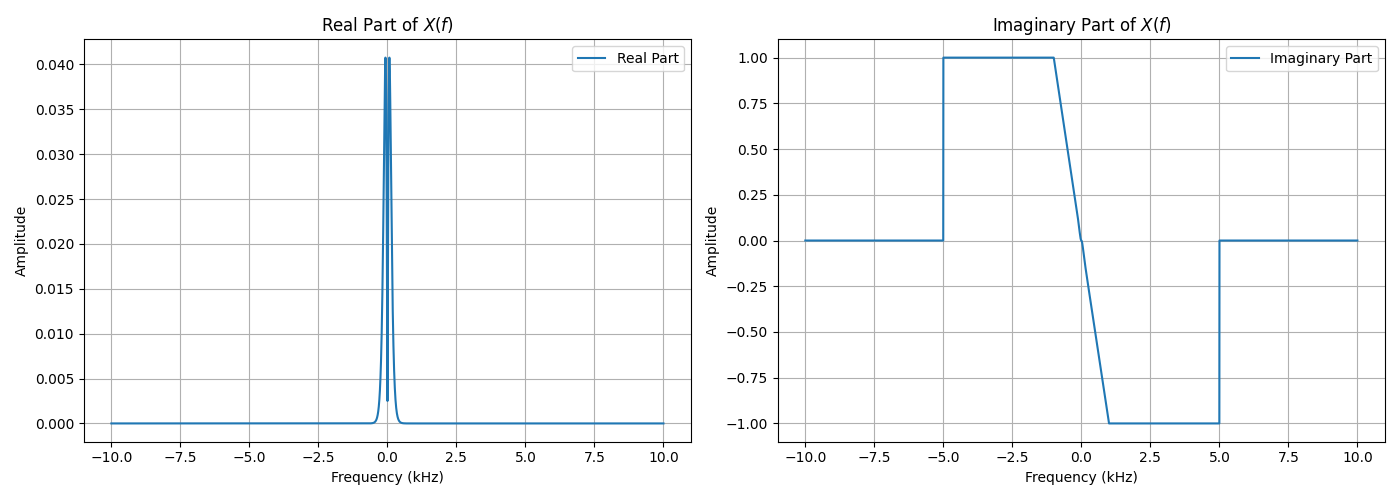
\includegraphics[width=0.49\textwidth]{fig/ex2_a_plot}
    \caption{Real and Imaginary Parts of $X(f)$}
    \label{fig:ex2_a_plot}
\end{figure}

%! Author = wolfram_e_laube
%! Date = 06.05.24

\item[(b)]
\subsection{Task (b): Spectrum of $x[n]$}

\subsubsection{Problem Statement}
Analyze and visualize the spectrum of the discrete-time signal $x[n]$, obtained by sampling the continuous-time signal $x(t)$ at a frequency $f_s$, and elucidate the effects of sampling including aliasing.

\subsubsection{Mathematical Formulation}
\begin{itemize}
    \item \textbf{Sampling Frequency $f_s = 8$ kHz}
    \item \textbf{Baseband:} $[-f_s/2, f_s/2]$ or $[-4 \text{ kHz}, 4 \text{ kHz}]$
\end{itemize}

The spectrum $X(f)$ repeats every $f_s$, illustrating the aliasing effects:
\[
\text{Extended Frequency Range for Visualization: } [-3f_s, 3f_s]
\]
\[
\text{Repeated Spectrum: } \text{tile}( |X(f)|, 3)
\]

\subsubsection{Discussion}
The plot of $x[n]$ shows how the spectrum repeats every $f_s$ and highlights the baseband where the original spectrum lies within the Nyquist range. This visualization demonstrates the aliasing effect, where parts of the spectrum outside the baseband overlap with those inside it.

\begin{figure}[h]
    \centering
    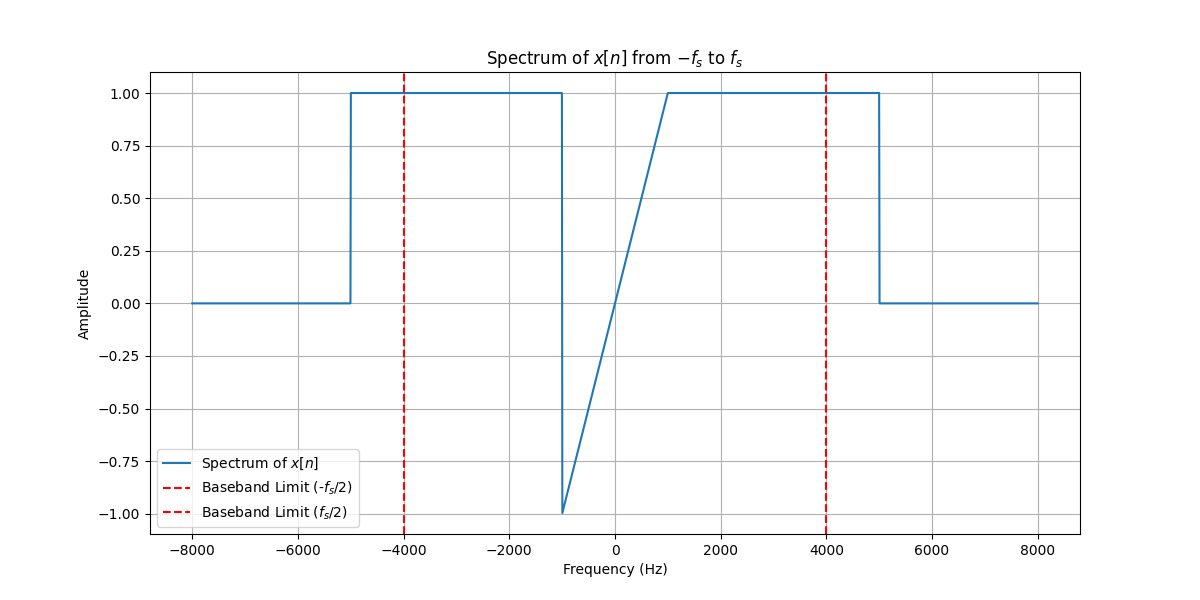
\includegraphics[width=0.49\textwidth]{fig/ex2_b_plot}
    \caption{Spectrum of \(x(t)\)}
    \label{fig:ex2_b_plot}
\end{figure}

\end{enumerate}

\end{aufgabe}

\begin{aufgabe}{Reconstruction (35\%)}

The discrete time signal \(x[n] = \sqrt{2} \cdot \sin \left(2 \pi \cdot \frac{1}{8} \cdot n\right)\) is converted to the analogue signal \(x(t)\) with a DAC which uses a clock frequency of \(8 \mathrm{kHz}\) and which converts a numerical value of 1 to \(1 \mathrm{~V}\).

\begin{enumerate}
    \item[(a)] Up to $20 \mathrm{kHz}$, list all positive frequencies which occur (in general) in $x(t)$.

    \item[(b)] The DAC implements a zero-order hold reconstruction.

    \begin{enumerate}
        \item[(1)] What is the power (in \(\mathrm{dB}\)) of the baseband sinewave (the sine at the lowest frequency).

        \item[(2)] What is the power (in \(\mathrm{dB}\)) of the first out-of-band sinewave (the sine with the second lowest frequency).
    \end{enumerate}

    \item[(c)] Qualitatively draw the spectrum of \(x(t)\) up to \(20 \mathrm{kHz}\). Delta pulses should be drawn with an arrow, the height of the arrow should indicate the weight of the delta-pulse.
\end{enumerate}

\textbf{Hints:}
\begin{itemize}
    \item The power of a sinewave with amplitude \(A\) is \(P=\frac{A^{2}}{2}\) (also see Parseval's theorem for periodic signals DSP\_02/27).

    \item The impulse response of a zero-order reconstruction filter is a rectangular pulse, its frequency response is thus given in \emph{DSP\_02/43}.

    \item When calculating the attenuation for the respective frequencies it should be noted that e.g. Matlab uses the normalized sinc function.
\end{itemize}

\hrule

\begin{enumerate}
\item[(a)]
\section*{Exercise 3 Task (a): Frequency Analysis of \(x(t)\)}

\subsection*{Objective}
This task involves identifying all positive frequencies up to 20 kHz in the analog signal \(x(t)\), derived from the discrete-time signal \(x[n]\) through a DAC operating at 8 kHz.

\subsection*{Methodology}
The discrete-time signal \(x[n] = \sqrt{2} \cdot \sin\left(2\pi \frac{1}{8} n\right)\) has a fundamental frequency \(f_0 = 1 \text{kHz}\) because it completes \(\frac{1}{8}\) of a cycle per sample, and the DAC operates at 8 kHz. The analysis focuses on the effects of sampling, which replicates the spectrum around multiples of the sampling frequency, leading to potential frequencies at:
\(f_0\),
\(f_s \pm f_0\),
\(2f_s \pm f_0\)
etc., where \(f_s\) is the sampling frequency (8 kHz).

\subsection*{Results}
The positive frequencies identified in \(x(t)\) and shown in Figure~\ref{fig:exercise3a_frequencies} are:
\begin{itemize}
\item 1 kHz (base frequency)
\item 7 kHz (\(8 \text{ kHz} - 1 \text{ kHz}\))
\item 9 kHz (\(8 \text{ kHz} + 1 \text{ kHz}\))
\item 15 kHz (\(16 \text{ kHz} - 1 \text{ kHz}\))
\item 17 kHz (\(16 \text{ kHz} + 1 \text{ kHz}\))
\end{itemize}

\begin{figure}[h]
    \centering
    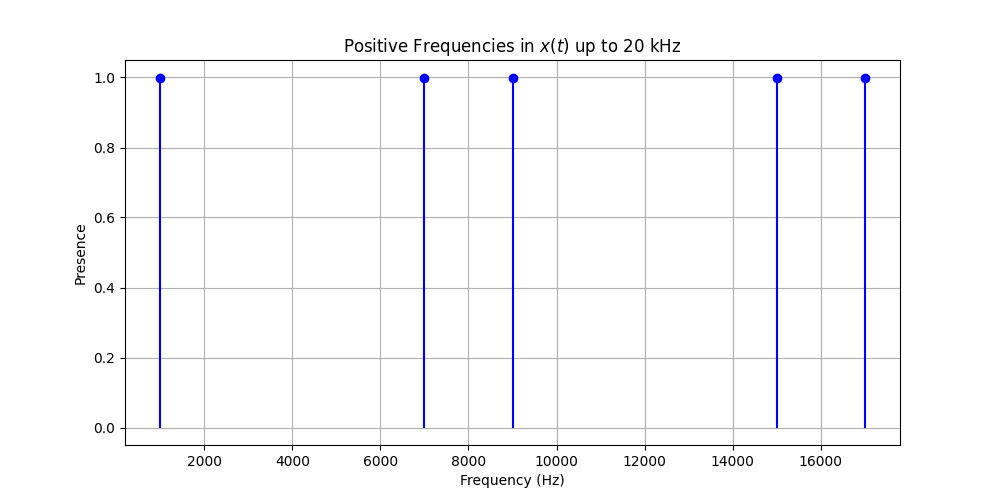
\includegraphics[width=0.8\textwidth]{fig/ex3_task_a_frequencies}
    \caption{Positive frequencies in \(x(t)\) up to 20 kHz}
    \label{fig:exercise3a_frequencies}
\end{figure}

\subsection*{Conclusion}
This detailed frequency analysis underscores the significance of understanding the effects of sampling on the signal's spectrum.
It aids in designing digital systems that effectively manage aliasing and maintain signal fidelity.

%! Author = wolfram_e_laube
%! Date = 02.04.24

\item [b)]
Plotting the Signals

Figure~\ref{fig:SignalPlot} shows two subplots, one for each frequency. In each subplot, it plots the original signal,
the time-delayed signal (in red dashed lines), and the phase-shifted signal (in green dot-dashed lines,
slightly transparent for better visibility).
The time-delayed and phase-shifted signals are expected to overlap completely,
demonstrating that a time delay is equivalent to a phase shift in the time domain.
\begin{figure}[!ht]
	\centering
	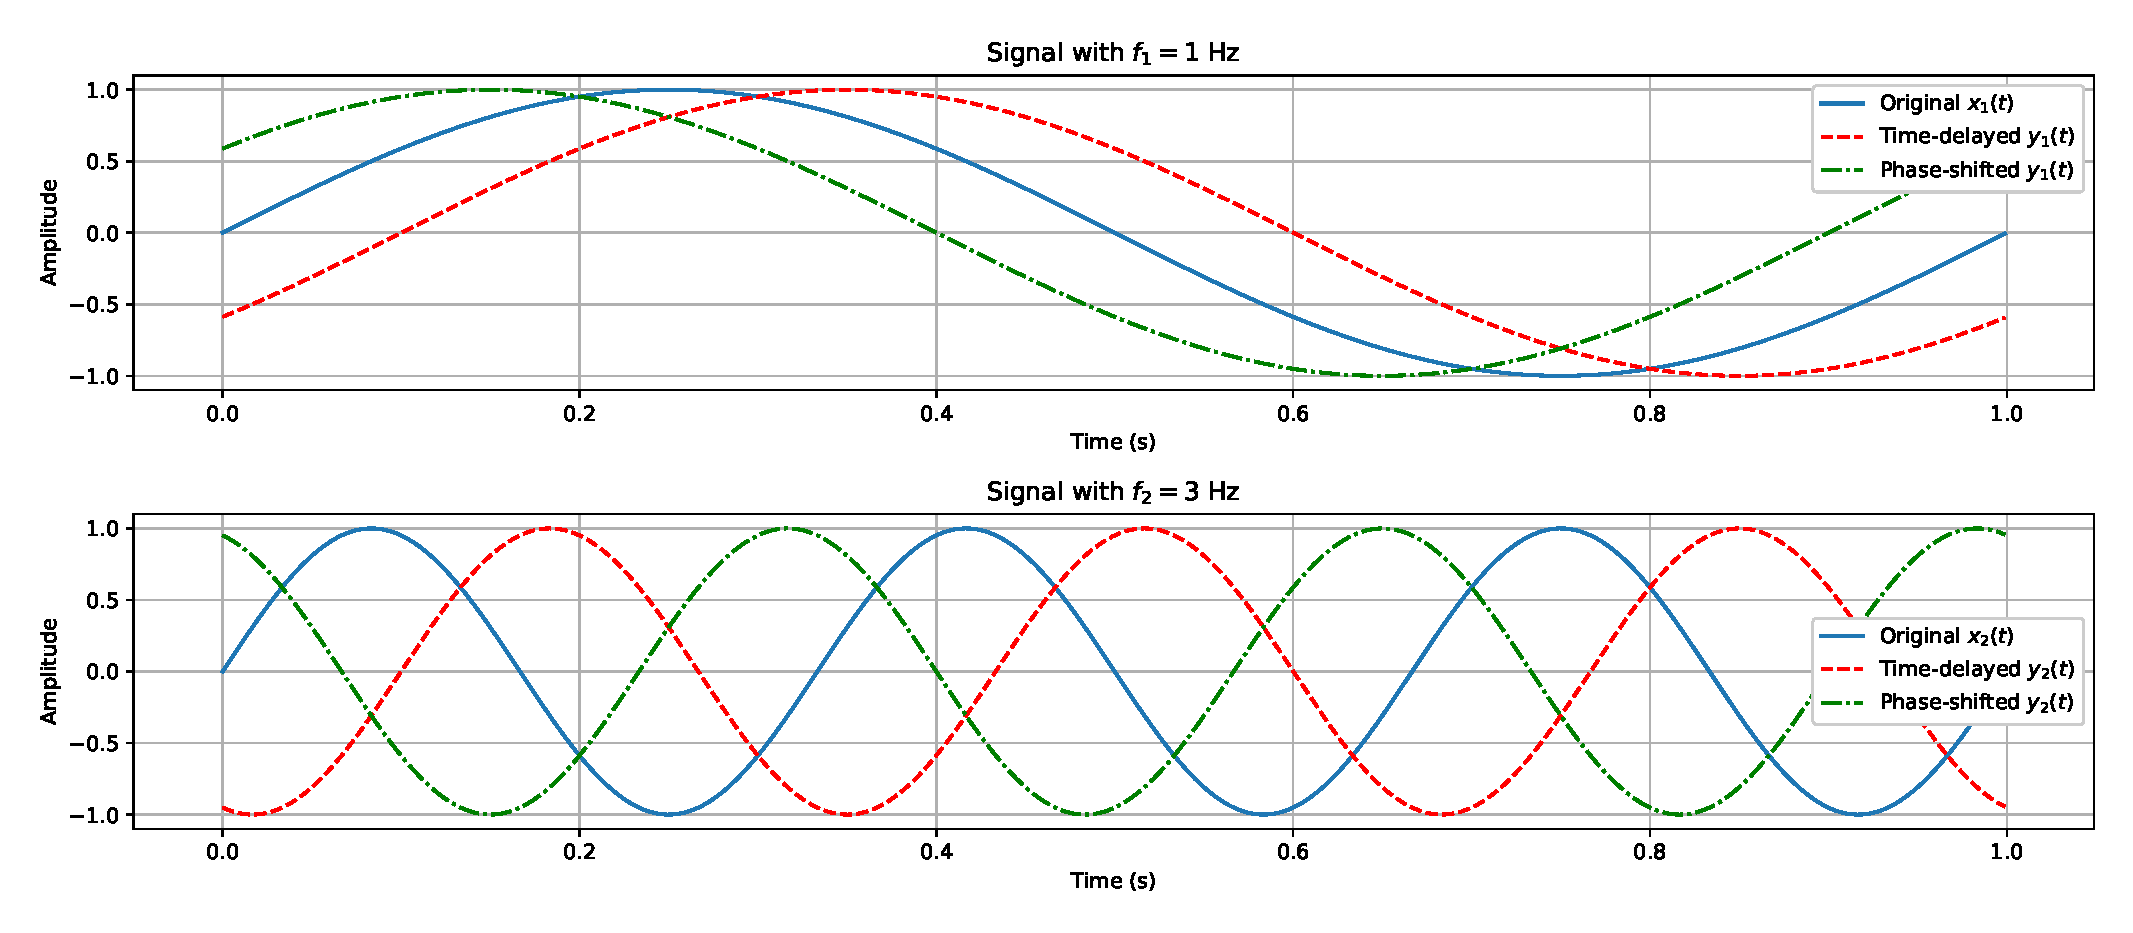
\includegraphics[width=18cm]{ex3_signal_plot.eps}
	\vspace{-0.3cm}
	\caption{Signal Plot.}
	\label{fig:SignalPlot}
	\vspace{-0.1cm}
\end{figure}



%! Author = wolfram_e_laube
%! Date = 06.05.24

\item[(c)]
Below is the Python code for this exercise:

\begin{verbatim}
import matplotlib.pyplot as plt

# Set up frequency range
fs = 8e3  # Sampling frequency
frequencies = [1e3, fs - 1e3]  # Example frequencies
weights = [1, 0.5]  # Example weights

# Plot spectrum
plt.figure()
for f, w in zip(frequencies, weights):
    plt.arrow(f / 1e3, 0, 0, w, head_width=0.2, head_length=0.05, color='blue', length_includes_head=True)
    plt.arrow(-f / 1e3, 0, 0, w, head_width=0.2, head_length=0.05, color='blue', length_includes_head=True)

plt.xlim(-20, 20)
plt.xlabel('Frequency (kHz)')
plt.ylabel('Weight')
plt.title('Qualitative Spectrum of $x(t)$')
plt.grid(True)
plt.show()
\end{verbatim}

\begin{figure}[h]
    \centering
    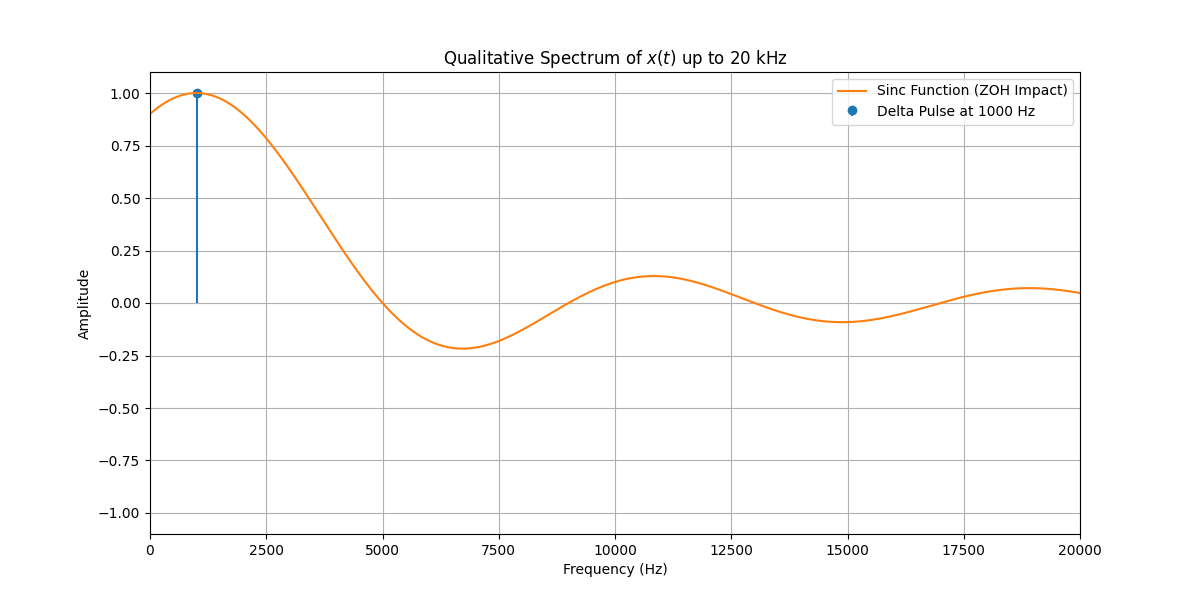
\includegraphics[width=0.49\textwidth]{fig/ex3_c_plot}
    \caption{Qualitative Spectrum of \(x(t)\)}
    \label{fig:ex3_c_plot}
\end{figure}

\end{enumerate}

\end{aufgabe}

\begin{aufgabe}{Signal Processing Onramp - BONUS (15\%)}
This task is optional (additional 15\%) and should help you to learn the basics of practical signal processing techniques in MATLAB.
You will find out how to use spectral analysis and filtering for preprocessing, analyzing, and extracting information from signal data.

For that, you need to carry out the full \emph{'Signal Processing Onramp course'}.
\footnote{\url{https://matlabacademy.mathworks.com/details/signal-processing-onramp/signalprocessing}}
To get the bonus points, you need to add the certificate to your protocol (you can download a pdf -
see \emph{'Share Certificate and Progress'}).
Also, you need to share your progress with my account (\texttt{matthias.wagner@jku.at}),
which can be done in the same tab.

%\hrule

%\begin{enumerate}
%\item[(a)]
\section{Normalized Radian Frequencies and Tolerances}

\subsection*{Problem Statement}
Specify the normalized radian frequencies for the passband \( \Omega_{\text{pass}} \) and the stopband \( \Omega_{\text{stop}} \), the passband tolerance \( \delta_{1} \), and the stopband tolerance \( \delta_{2} \).

Given:
\begin{itemize}
    \item Passband cutoff frequency: \( f_{\text{pass}} = 3.4 \text{kHz} \)
    \item Stopband cutoff frequency: \( f_{\text{stop}} = 4 \text{kHz} \)
    \item Allowed ripple in the passband: \( \pm 5\% \)
    \item Minimum stopband attenuation: \( 45 \text{dB} \)
    \item Sampling frequency: \( f_s = 20 \text{kHz} \)
\end{itemize}

\subsection*{Theoretical Background}
Normalized radian frequencies are calculated using the formula:
\[ \Omega = \frac{2\pi f}{f_s} \]
where \( f \) is the frequency in Hz and \( f_s \) is the sampling frequency in Hz.

Passband tolerance \( \delta_1 \) is the maximum allowed deviation from the desired gain (1) in the passband, given as a percentage.

Stopband tolerance \( \delta_2 \) is derived from the minimum stopband attenuation, given in decibels (dB). It is calculated using the formula:
\[ \delta_2 = 10^{-\frac{A}{20}} \]
where \( A \) is the attenuation in dB.

\subsection*{Mathematical Derivation}

\subsubsection*{Normalized Radian Frequencies}
\begin{itemize}
    \item Passband cutoff frequency:
    \[
    \Omega_{\text{pass}} = \frac{2\pi \times 3400}{20000} = 0.34\pi
    \]
    \item Stopband cutoff frequency:
    \[
    \Omega_{\text{stop}} = \frac{2\pi \times 4000}{20000} = 0.4\pi
    \]
\end{itemize}

\subsubsection*{Passband Tolerance \( \delta_1 \)}
Given \( \pm 5\% \) ripple in the passband, the tolerance is:
\[
\delta_1 = 0.05
\]

\subsubsection*{Stopband Tolerance \( \delta_2 \)}
Given a minimum stopband attenuation of \( 45 \text{dB} \):
\[
\delta_2 = 10^{-\frac{45}{20}} = 10^{-2.25} \approx 0.00562
\]

\subsection*{Conclusion}
The normalized radian frequencies and tolerances for the lowpass filter are:
\begin{itemize}
    \item Passband cutoff frequency \( \Omega_{\text{pass}} = 0.34\pi \)
    \item Stopband cutoff frequency \( \Omega_{\text{stop}} = 0.4\pi \)
    \item Passband tolerance \( \delta_1 = 0.05 \)
    \item Stopband tolerance \( \delta_2 = 0.00562 \)
\end{itemize}

%%! Author = wolfram_e_laube
%! Date = 16.04.24

\item[(b)]
The magnitude and phase response of the DTFT is plotted using the following Python code:

\begin{verbatim}
import matplotlib.pyplot as plt
import numpy as np

# Given sequence parameters
n = np.arange(-10, 11)  # Since x[n] is nonzero for n between -10 and 10
x = (0.8)**np.abs(n)

# Frequency vector
w = np.linspace(-np.pi, np.pi, 1000)

# Compute DTFT
X = dtft(x, n, w)

# Plot magnitude and phase response
plt.figure(figsize=(14, 6))

# Magnitude response subplot
plt.subplot(2, 1, 1)
plt.plot(w, np.abs(X))
plt.title('Magnitude Response of $X(e^{j\Omega})$')
plt.xlabel('$\Omega$')
plt.ylabel('|X|')
plt.grid()

# Phase response subplot
plt.subplot(2, 1, 2)
plt.plot(w, np.angle(X))
plt.title('Phase Response of $X(e^{j\Omega})$')
plt.xlabel('$\Omega$')
plt.ylabel('Phase (radians)')
plt.grid()

plt.tight_layout()
plt.show()
\end{verbatim}

This code segment uses Matplotlib to create the plots for the magnitude and phase responses
of the DTFT computed for a discrete sequence.

\begin{figure}[h]
\centering
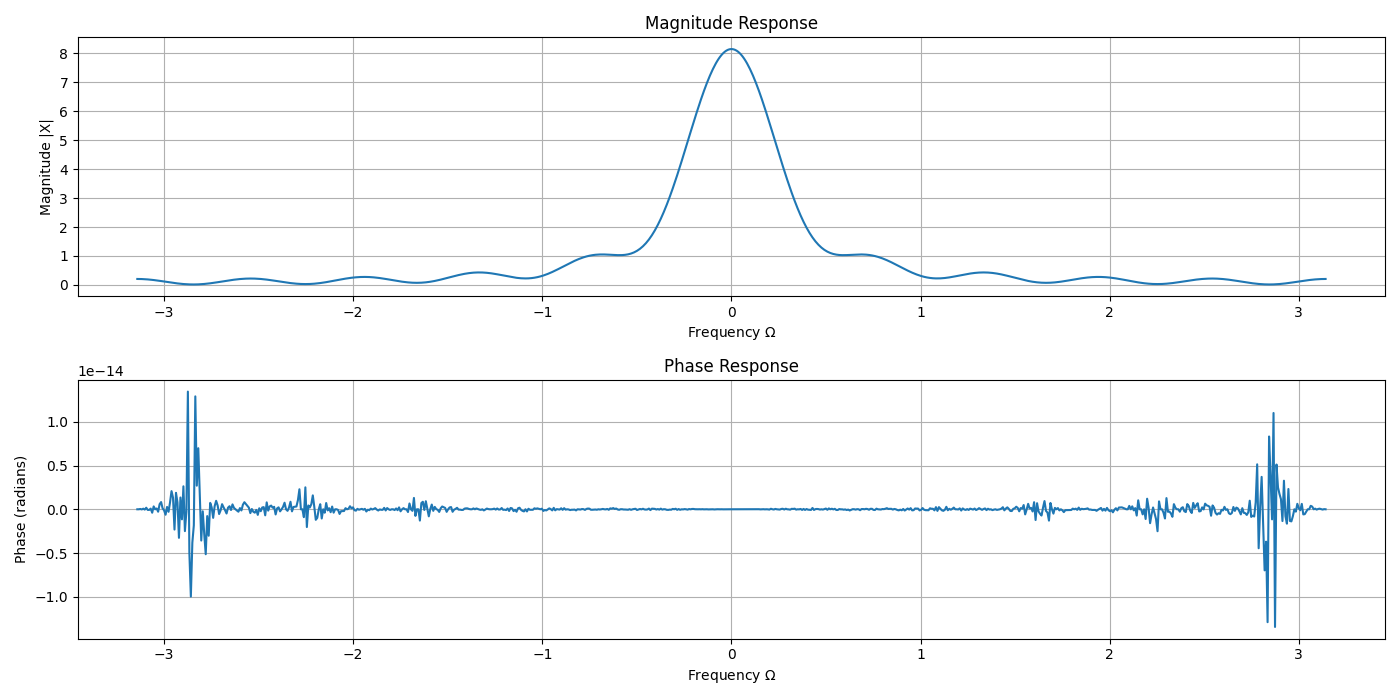
\includegraphics[width=\textwidth]{fig/ex4_b_plot}
\caption{Magnitude and phase of DTFT}
\label{fig:ex4_b_plot}
\end{figure}

%\item[(a)]
\section*{Task (a)}

\subsection*{Problem Statement}
% TODO insert problem statement here

\subsection*{Theoretical Background}
% TODO insert theoretical here

\subsection*{Mathematical Derivation}
% TODO insert mathematical derivation here

\subsection*{Python Implementation and Plot}
% TODO insert plot description here
The plot Figure~\ref{fig:ex1_a_plot} below illustrates these this

% TODO insert plot here
\begin{figure}[h]
    \centering
    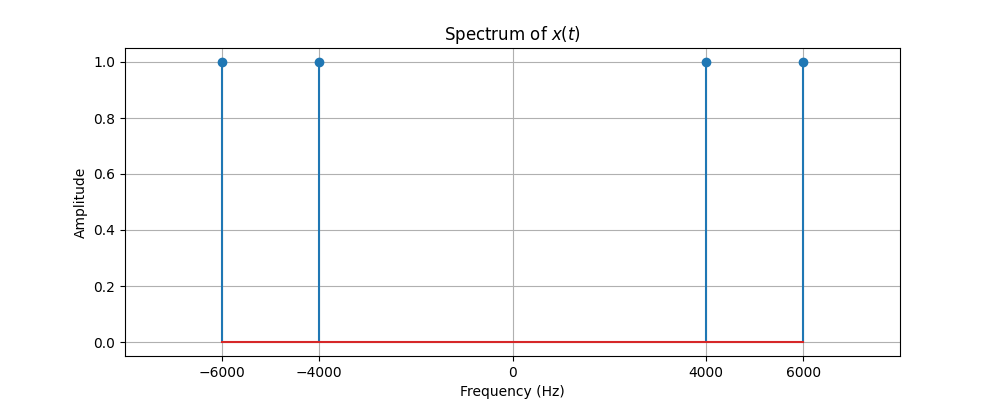
\includegraphics[width=0.8\textwidth]{fig/ex1_a_plot}
    \caption{Exercise 1 Task (a)}
    \label{fig:ex1_a_plot}
\end{figure}

\subsection*{Conclusion}
%\end{enumerate}

\end{aufgabe}


\end{document}
